% !TEX TS-program = pdflatex
% !TEX root = ../tesi.tex

%************************************************
\chapter{Electroacoustic Composition Workflow}
\label{chp:fundamentals}
%************************************************

As already said, electroacoustic sounds are made by a computational composing instrument written in Wolfram Language. The code is written by my electroacoustic composition teacher \textbf{Francesco Scagliola} in a computing system called \textbf{Mathematica}.
	
	\section{Computing enviroment}
	But What does this code do?
	In order to understand it, it's need to talk about what \textbf{CSound} is and what it can do.
	
		\subsection{CSound}
		Csound is a software synthesis and audio programming language used for sound synthesis, composition, and signal processing. It was originally developed by Barry Vercoe at the Massachusetts Institute of Technology (MIT) in the 1980s.
		Csound provides a powerful and flexible environment for \textbf{creating} and \textbf{manipulating} digital audio. It offers a wide range of built-in sound synthesis and processing modules, as well as the ability to create custom instruments and effects using its programming language. With Csound, users can design complex and intricate sounds, create generative music, and perform real-time audio processing.
		Csound can be used on various operating systems, including Windows, macOS, and Linux. It is widely used by musicians, composers, sound designers, and researchers in the field of computer music and audio programming.
		Csound it's a language that works in different compilers: just as it is possible to write a LaTex document in TexStudio or MikTex, it's possible to write CSound code in compilers such as WinxSound and CSoundQT
		Overall, Csound provides a powerful toolset for sound synthesis and audio programming, allowing users to explore and create a wide range of possibilities.
		
		\subsection{Connection between Mathematica and Csound}
		The instrument written by Francesco Scagliola in Wolfram allows the composer to connect Mathematica to Csound.
		The functions written inside the Wolfram code create different CSound codes which correspond to different instruments, each with a different use. some of these are illustrated in the following paragraphs
		
		\paragraph{Additive Synthesis} Let's start with the simplest.
		First of all, what additive synthesis is and how does it work?
		Additive synthesis in sound design involves combining multiple waves, each with its frequency and amplitude, to create complex and rich sounds. By adjusting the parameters of these waves, intricate timbres can be achieved. This technique allows sound designers to build harmonically rich textures, simulate real-world instruments, and create unique sonic atmospheres.
		Francesco Scagliola wrote some functions that allow the user to write a large number of lines of code in the score of a CSound code with only one line of code using 3/4 functions. In the case of additive synthesis, few computational calculations are performed. 
		The structure of the code recalls the tool for additive synthesis in CSound and, once the orchestra of the code has been set, in the score section, by modifying the values, create tables that write values ​​in series in the synthesis parameters sample by sample. Once compiled, the code will return a CSound code, the file.wave generated by compiling the Csound code and a copy of the Mathematica code.
		
		\begin{figure}[h]
			\begin{center}
				\begin{code}
					</CsInstruments>
					
					<CsScore>
					
					f 1 0 1048576 11  1 
					f 2 0 1048576 10  10 2
					f 3 0 1048576 10  10 0 2
					f 4 0 1048576 10  10 0 0 2
					f 5 0 1048576 10  10 0 0 0 2
					f 6 0 1048576 10  10 0 0 0 0 2
					f 7 0 1048576 10  10 0 0 0 0 0 2
					f 8 0 1048576 10  10 0 0 0 0 0 0 2
					f 9 0 1048576 10  10 0 0 0 0 0 0 0 2
					f 10 0 1048576 10 10 0 0 0 0 0 0 0 0 2
					f 11 0 1048576 10 10 0 0 0 0 0 0 0 0 0 2
					f 12 0 1048576 10 10 0 0 0 0 0 0 0 0 0 0 2
					f 13 0 1048576 10 10 0 0 0 0 0 0 0 0 0 0 0 2
					f 14 0 1048576 10 10 0 0 0 0 0 0 0 0 0 0 0 0 2
					f 15 0 1048576 10 10 0 0 0 0 0 0 0 0 0 0 0 0 0 2
					f 16 0 1048576 10 10 0 0 0 0 0 0 0 0 0 0 0 0 0 0 2
					f 17 0 1048576 10 10 0 0 0 0 0 0 0 0 0 0 0 0 0 0 0 2
					f 18 0 1048576 10 10 0 0 0 0 0 0 0 0 0 0 0 0 0 0 0 0 2
					f 19 0 1048576 10 10 0 0 0 0 0 0 0 0 0 0 0 0 0 0 0 0 0 2
					f 20 0 4096 7 -1 2048 1 2048 -1; Triangolare
					f 21 0 4096 7 -1 2048 -1  1 1  2047 1; Quadra
					f 101 0 1048576 10 2 1 .333 .5 0 .1666 0 .25 0 0 0 .083333 0 0 0 .125 0 0 0 0 0 0 0 .16666 0 0 0 0 0 0 0 .25 0 0 0 0 0 0 0 0 0 0 0 0 0 0 0 0 0 0 0 0 0 0 0 0 0 0 0 0 0 0 0 1 .5 .333 .25 0 .1666 0 .125 0 0 0 .083333 0 0 0 .0625 0 0 0 0 0 0 0 .16666 0 0 0 0 0 0 0 .25 1 1 1 1 1 1 1 1 1 1 1 1 1 1 1 1 1 1 1 1 1 1 1 1 1 1 1 1 1 1 1 10
					f 200 0 1048576 30 21 1 7
				\end{code}
				\caption{By computing the wolfram code cell of additive synthesis, a CSound code is generated. In this figure ih shown the score of a generated CSound code that include a simple additive synthesis tool in his orchestra}
			\end{center}
		\end{figure}
		
		\textbf{Francesco Scagliola} wrote several functions that, used in different ways, allowed him to create more tools for additive synthesis. the main are:
		
		\begin{compactitem}
			\item Simple additive synthesis that allows to combine simple sine waves in order create different timbres
			\item Polyphonic additive synthesis tool that allows to layer numerous sine waves to create complex polyphonic chords and textures
			\item Rythm tools that allows to create dense rhythms, with short sine wave with a short attack time, that never repeat identically over time
			\item A complex tool that allows to create very intresting cluster and crescendo by layering sine waves
		\end{compactitem}
		
		\paragraph{Sampler} This tools are the most used in this work.
		This tool combines functions that allow to recall a sound source external to the code and sample it with different sampling techniques:
		
			\begin{compactitem}
				\item \textbf{Granular synthesis} in sound design involves breaking down audio samples into tiny grains with different attack-time and envelopes in order to manipulate them individually. These grains, typically a few milliseconds long, can be modified in terms of pitch, duration, and spatial placement. By rearranging and layering these grains in various ways, intricate and complex textures can be created, allowing for the transformation of sounds in unique and imaginative ways.
				\item \textbf{Time stretching} is a technique in sound design that involves altering the duration of an audio sample without affecting its pitch. It allows for the manipulation of the playback speed of a sound while maintaining its original tonality. By stretching or compressing the time domain of a sample, sound designers can create slow-motion effects, extend or shorten musical phrases, or match the tempo of different audio elements.
			\end{compactitem}
		
		In this chase, the CSound code score includes also the name of the external file sampled:
		
			\begin{figure}[h]
				\begin{center}
					\begin{code}
						i          1.                    0.                    1.                    1.6         	"CM3 (9).wav"          1.                    0.                    0.01                  0.1951089103
						i          1.                    0.0038222564          1.                    0.1         	"CM3 (9).wav"         -1.                    0.0001052632          0.01                  0.8220174094
						i          1.                    0.025444204           1.                    0.1         	"CM3 (9).wav"          1.                    0.0002105263          0.01                  0.4180911663
						i          1.                    0.0470661515          1.                    0.1         	"CM3 (9).wav"         -1.                    0.0003157895          0.01                  0.2080246873
						i          1.                    0.050888408           1.                    0.1         	"CM3 (9).wav"          1.                    0.0004210526          0.01                  0.8028244885
						i          1.                    0.0547106644          1.                    0.1         	"CM3 (9).wav"         -1.                    0.0005263158          0.01                  0.6040055079
						i          1.                    0.0763326119          1.                    0.1         	"CM3 (9).wav"          1.                    0.0006315789          0.01                  0.9605029126
						i          1.                    0.0801548684          1.                    0.1         	"CM3 (9).wav"         -1.                    0.0007368421          0.01                  0.1977322379
						i          1.                    0.0839771248          1.                    0.1         	"CM3 (9).wav"          1.                    0.0008421053          0.01                  0.7952956606
						i          1.                    0.0877993812          1.                    0.1         	"CM3 (9).wav"         -1.                    0.0009473684          0.01                  0.8338141507
					\end{code}
					\caption{The values shown sets the attack time, the duration time, the time point in wich the audio file must be sampled, the time stretching percentage, the amplitude, the name of audio file and the spazialization. Grouped in two lines of code for each sampling action}
				\end{center}
			\end{figure}
		
		As the same as the additive synthesis code, for the sampler code there are several tools that make different type of sampling, the main are:
		
			\begin{compactitem}
				\item Simple sampling tool: allows to chose an audio file and to sample it.
				\item Multiple sampling tool: allows to chose multiple audio files and layering them in a more intresting audio flow
				\item Tuning tool: allows to make a time-stretching by tuning samples in order to make them sound in a specific tune
				\item Granular Synthesis
			\end{compactitem}
		
		\paragraph{Subtractive Synthesis} is a sound design technique that involves starting with a rich and harmonically complex waveform (like white or pink noise) and then shaping the sound by removing or filtering out specific frequencies using filters. By adjusting the cutoff frequency, resonance, and filter types, sound designers can sculpt the timbre and shape of the sound.
		This code is written to allow the user to compute electroacoustic gestures with this technique, filtering white noise. It recalls the filtering tools in CSound and a tool that generates white noise. To generate white noise in CSound:
		
		\newpage
		
		\begin{code}
			<CsInstruments>
			instr 1
			kDuration = p3
			aNoise    noise kDuration
			outs aNoise, aNoise
			endin
			</CsInstruments>
			<CsScore>
			i 1 0 1
			e
			</CsScore>
		\end{code}
		
		In the code shown above, an instrument for generating white noise is written by the function aNoise, which tells to the calculator to generate white noise for duration "p3". At the end of the syntax of the Instrument, the score begins. In the first line of the score is written "i 1 0 1" which means "recall the instrument 1 defined in the orchestra and generate 1 sample"
		
	\section{Wwise as an instrument}
	Now born a spontaneous question. The code written by Francesco Scagliola in Wolfram was used as a compositional tool. In this work, Wwise is used as a formal editing and management tool.
	But is it possible to use the middleware Wwise as a compositional tool? Is it possible to control its functions using external programs or languages ​​such as Touch Designer, MaxMsp, Csound or Mathematica?
	To explore the possibilities in this regard, it is necessary to understand where Wwise receives information from.
	
		\subsection{Sound.cpp}
		The Wwise project of Cube organized his events, actor-mixer hierarchy, and sound banks to work with triggers that come from the video game while the player is making actions. But how do they communicate? In the C++ scripts of the game engineering, there is one called "sound. ccp" in which are written the rules for the communication between Wwise and Cube: the function written in this code makes a connection between the name of the trigger that comes in input from the output of the game engineering, and the name of the trigger in output that goes to the input of Wwise, which take this trigger in the routed events in the project which calls the external file. wave and make the computed interpolation on it to create the soundbanks. In sound. ccp is written also a function that includes the soundbank exported from the Wwise project into the final file.exe of the game computed.
		So, the answer to the question "is it possible to use Wwise as a compositional tool?" is "yes", but writing functions inside a code that, in this case, correspond to "sound. ccp", links the Wwise events to an external trigger. This trigger may come from another control environment, such as MaxMsp or Wolfram Mathematica.
		
		\begin{figure}[h]
			\begin{center}
				\begin{code}
					#include "cube.h"
					
					#undef min
					#undef max
					
					#include <algorithm>
					#include <list>
					
					#include <AK/SoundEngine/Common/AkSoundEngine.h>
					#include <AK/SoundEngine/Common/AkModule.h>
					#include <AK/MusicEngine/Common/AkMusicEngine.h>
					#include <AK/Tools/Common/AkLock.h>
					#include <AK/Tools/Common/AkMonitorError.h>
					#include <AK/Tools/Common/AkPlatformFuncs.h>
					#include <AkDefaultIOHookBlocking.h>
					
					#ifndef AK-OPTIMIZED
					#include <AK/Comm/AkCommunication.h>
					#endif
					
					static const AkGameObjectID LISTENER-ID = 10001;
					
					#include <AK/Plugin/AllPluginsFactories.h>
				\end{code}
				\caption{Header of the code sound.ccp}
			\end{center}
		\end{figure}
	

\begin{comment}
\begin{code}
\documentclass[\meta{\dots\unkern}]{scrreprt} % or scrbook or scrartcl

\usepackage[\meta{\dots\unkern}]{classicthesis}
\usepackage{arsclassica}

\begin{document}
\dots
\end{document}
\end{code}

For example, this document has been produced with the following code:
\begin{code}
\documentclass[a4paper,twoside,openright,titlepage,
               headinclude,footinclude,BCOR5mm,
               numbers=noenddot,cleardoublepage=empty,
               tablecaptionabove]{scrreprt}

\usepackage{\meta{\dots\unkern}}
\usepackage{subfig}
\usepackage[eulerchapternumbers,subfig,beramono,eulermath,pdfspacing]%
           {classicthesis}
\usepackage{arsclassica}

\begin{document}
\dots
\end{document}
\end{code}

It is recommended to use the \optname{beramono} and \optname{eulerchapternumbers} options together with \arsclassica.



\section{Style}

The typographical style achieved with \arsclassica{} differs from \classicthesis{} in the following points:
\begin{itemize}
\item use of Iwona font, by Janusz Nowacki, for the sectioning unit titles (chapters, sections, subsections, sub-subsections, paragraphs and subparagraphs), for the description list labels, the headlines and the caption labels (\classicthesis{} doesn't use any sans serif font);
\item customized chapter numbers;
\item semi-transparent headlines; the headlines are separated from the page number by a small rule;
\item caption labels in boldface (\classicthesis{} doesn't use any boldface font);
\item itemize lists with semi-transparent bullets.
\end{itemize}

\arsclassica{} is designed  to provide a ready-to-use typographical style: for this reason it has no loading options and it is \emph{not} configurable or customizable in any way. If you change the previous settings, you'll risk to destroy the balance of the style, so it is \emph{highly recommended} to keep them unchanged.

One of the principles of \LaTeX{} is that it allows the author to take no interest in the typographical questions, permitting him to focus only on the structure and the contents of his document. This fact should always be kept in mind: using a style written by others, the user accepts all the typographical settings chosen for him by the author of the style, and he isn't forced to study typography to fine-tune the layout of his publications. This is the case of \arsclassica{} too: if you change its settings, you'll deny this philosophy and, consequently, you'll have to study (a lot of) typography to achieve acceptable results.

The style achieved with \arsclassica{} is \emph{not} therefore configurable or customizable. The typographical style is very personal: if you like this package and find attractive the idea to take no interest in the problem of the style definition, then you'll use \arsclassica{} with satisfaction; otherwise, if you have different needs or you aren't satisfied with the layout of the package, then you should try other classes or packages, even building your own style.



\section{Important}

To write a document according to the \arsclassica{} style, you have to follow some very simple rules.
\begin{itemize}
\item Don't change \emph{for any reason} the \arsclassica{} settings (fonts, text body size, colors, \dots).
\item The sectioning unit titles (chapters, section, subsections, \dots) have to be \emph{one line long}, possibly in \emph{plain text} (no symbols, formulas or code fragments). If you have titles longer than one line, try and rephrase them: you can almost always do it.
\item In the table of contents and in the list of tables and figures, captions have to be \emph{one line long}, possibly in \emph{plain text}. Use the optional argument of sectioning commands and of \cmdname{caption}, if necessary.
\item Don't use \optname{tocaligned} and \optname{dottedtoc} options of \classicthesis: the default table of contents does the job very well (see the documentation of \classicthesis{} for a nice discussion of this point).
\item Don't use vertical or double rules in your tables (see the documentation of \pkgname{booktabs}).
\item Use footnotes and margin notes very sparingly.
\item If your document includes graphs and plots, draw them using \LaTeX{} (by \pkgname{Ti\emph{k}Z} and \pkgname{pgfplots}, for example) and not an external software. This is the only way to get the best typographical outcome.
\end{itemize}



\section{Examples}

%\begin{figure}
%\centering
%\subfloat[Asia personas duo]
%{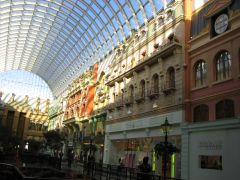
\includegraphics[width=.45\columnwidth]{Lorem}} \quad
%\subfloat[Pan ma signo]
%{\label{fig:example-b}%
%
\includegraphics[width=.45\columnwidth]{Ipsum}} \\
%\subfloat[Methodicamente o uno]
%{
\includegraphics[width=.45\columnwidth]{Dolor}} \quad
%\subfloat[Titulo debitas]
%{
\includegraphics[width=.45\columnwidth]{Sit}}
%\caption[Tu duo titulo debitas latente]{Tu duo titulo debitas latente}
%\label{fig:example}
%\end{figure}

Please note that the content of this section is just some dummy text. It isn't a real language.

Lorem ipsum dolor sit amet, consectetuer adipiscing elit. Ut purus elit, vestibulum ut, placerat ac, adipiscing vitae, felis. Curabitur dictum gravida mauris.

\subsection*{A subsection}

\lipsum[2]

\subsubsection*{A sub-subsection}

\lipsum[7]

\paragraph{A paragraph}
Lorem ipsum dolor sit amet, consectetuer adipiscing elit. Ut purus elit, vestibulum ut, placerat ac, adipiscing vitae, felis. Curabitur dictum gravida mauris. Nam arcu libero, nonummy eget, consectetuer id, vulputate a, magna.

\paragraph{Another paragraph}
Cras nec ante, pellentesque a nulla, cum sociis natoque penatibus et magnis dis parturient montes, nascetur ridiculus mus. Aliquam tincidunt urna

\bigskip

Donec aliquet, tortor sed accumsan bibendum, erat ligula aliquet magna, vitae ornare odio metus a mi. Morbi ac orci et nisl hendrerit mollis. Suspendisse ut massa. Cras nec ante. Pellentesque a nulla. Cum sociis natoque penatibus et magnis dis parturient montes, nascetur ridiculus mus. Aliquam tincidunt urna.

\begin{description}
\item[Mane] Lorem ipsum dolor sit amet, consectetuer adipiscing elit.
\item[Tekel] Ut purus elit, vestibulum ut, placerat ac, adipiscing vitae, felis. Curabitur dictum gravida mauris.
\item[Fares] Nam arcu libero, nonummy eget, consectetuer
id, vulputate a, magna.
\end{description}

\begin{table}
\caption{Lorem ipsum dolor sit amet}
\centering
\begin{tabular}{ll}
\toprule
\textbf{Alkaloid} & \textbf{Origin} \\
\midrule
atropine & belladonna \\
morphine & poppy \\
nicotine & tobacco \\
\bottomrule
\end{tabular}
\end{table}

Suspendisse vel felis. Ut lorem lorem, interdum eu, tincidunt sit amet, laoreet vitae, arcu. Aenean faucibus pede eu ante. Praesent enim elit, rutrum at, molestie non, nonummy vel, nisl. Ut lectus eros, malesuada sit amet, fermentum eu, sodales cursus, magna. Donec eu purus. Quisque vehicula, urna sed ultricies auctor, pede lorem egestas dui, et convallis elit erat sed nulla.

\subsection*{Some formulas}

Una formula in linea viene incorporata nel testo: $\lim_{n \to \infty}\sum_{k=1}^n \frac{1}{k^2} = \frac{\pi^2}{6}$, per esempio. Come si osserva, \LaTeX{} fa \emph{il possibile} per comprimerla e modificare il meno possibile l'interlinea nel capoverso che la contiene.
Una formula in display viene invece composta da \LaTeX{} su linee a parte, separate dal contesto con adeguati spazi bianchi per metterla in mostra e farla risaltare sulla pagina.
\begin{equation}
\lim_{n \to \infty}\sum_{k=1}^n \frac{1}{k^2}= \frac{\pi^2}{6}
\end{equation}
Come si osserva, ora la formula risulta centrata, non compressa, e tutti i suoi elementi occupano il giusto spazio con un risultato finale di grande respiro.

Integer tempus convallis augue. Etiam facilisis. Nunc elementum fermentum wisi. Aenean placerat. Ut imperdiet, enim sed gravida sollicitudin, felis odio placerat quam, ac pulvinar elit purus eget enim.

\begin{equation}
\int_a^{a+T}f(x)\,dx= \int_0^T f(x)\,dx
\qquad
\oint f(z)\,dz=2\pi i
\end{equation}

Nulla malesuada porttitor diam. Donec felis erat, congue non, volutpat at, tincidunt tristique, libero. Vivamus viverra fermentum felis. Donec non- ummy pellentesque ante.

\begin{equation}
f(x_1,\dots,x_n)=  \prod_{k=1}^n x_k
\qquad
\sum_{k=1}^n x_k^2=1
\qquad
\biggl(\sum_n x_n^2\biggr)^{1/2}
\end{equation}

\lipsum[2]

\begin{equation}
\begin{bmatrix}
a_{11} & \dots & a_{1n} \\
a_{21} & \dots & a_{2n} \\
\hdotsfor{3} \\
a_{n1} & \dots & a_{nn}
\end{bmatrix}
\end{equation}

\lipsum[4]

\begin{equation}
\lim_{x\to 0}
\frac{\sin x}{x}=1 \qquad
\lim_{n\to +\infty}f_n=\delta
\end{equation}

Fusce mauris. Vestibulum luctus nibh at lectus. Sed bibendum, nulla a faucibus semper, leo velit ultricies tellus, ac venenatis arcu wisi vel nisl. Vestibulum diam.

\begin{equation}
n!=
\begin{cases}
1       & \text{if $n=0$} \\
n(n-1)! & \text{if $n\ge 1$}
\end{cases}
\end{equation}

Ut lectus eros, malesuada sit amet, fermentum eu, sodales cursus, magna. Donec eu purus. Quisque vehicula, urna sed ultricies auctor, pede lorem egestas dui, et convallis elit erat sed nulla. Donec luctus. Curabitur et nunc. Aliquam dolor odio, commodo pretium, ultricies non, pharetra in, velit.

\begin{equation}
x_G=
\frac{\displaystyle
      \sum_{i=1}^n m_ix_i}
{\displaystyle\sum_{i=1}^n m_i}
\end{equation}

\lipsum[6]

\begin{equation}
\kappa =\frac{\xi}{E_{\textrm{max}}}
\qquad
E_{\textup{max}} =\frac{2 m_{\textup{e}} \beta^2\gamma^2 }{1 +2\gamma m_{\textup{e}}/m_{\textrm{x}} + ( m_{\textup{e}}/m_{\textup{x}})^2}
\end{equation}

\lipsum[8]
\end{comment}